% GPTBlock 内部结构图 — OLMo 2 post-norm + RoPE + QK-Norm + SwiGLU
% 编译: pdflatex gptblock.tex   (或 latexmk -pdf)
% 嵌入论文: % GPTBlock 内部结构图 — OLMo 2 post-norm + RoPE + QK-Norm + SwiGLU
% 编译: pdflatex gptblock.tex   (或 latexmk -pdf)
% 嵌入论文: % GPTBlock 内部结构图 — OLMo 2 post-norm + RoPE + QK-Norm + SwiGLU
% 编译: pdflatex gptblock.tex   (或 latexmk -pdf)
% 嵌入论文: % GPTBlock 内部结构图 — OLMo 2 post-norm + RoPE + QK-Norm + SwiGLU
% 编译: pdflatex gptblock.tex   (或 latexmk -pdf)
% 嵌入论文: \input{figures/gptblock.tex}
%
% 对应 src/mdlic/models/layers.py:GPTBlock (line 366)
%   x = x + DropPath(RMSNorm(Attn(x)))    -- OLMo 2 post-norm，注意 Norm 在 sublayer 之后
%   x = x + DropPath(RMSNorm(FFN(x)))
\documentclass[tikz,border=8pt]{standalone}
\usepackage{tikz}
\usepackage{amsmath,amssymb}
\usetikzlibrary{positioning,arrows.meta,calc,fit,backgrounds,shapes.geometric}

\begin{document}
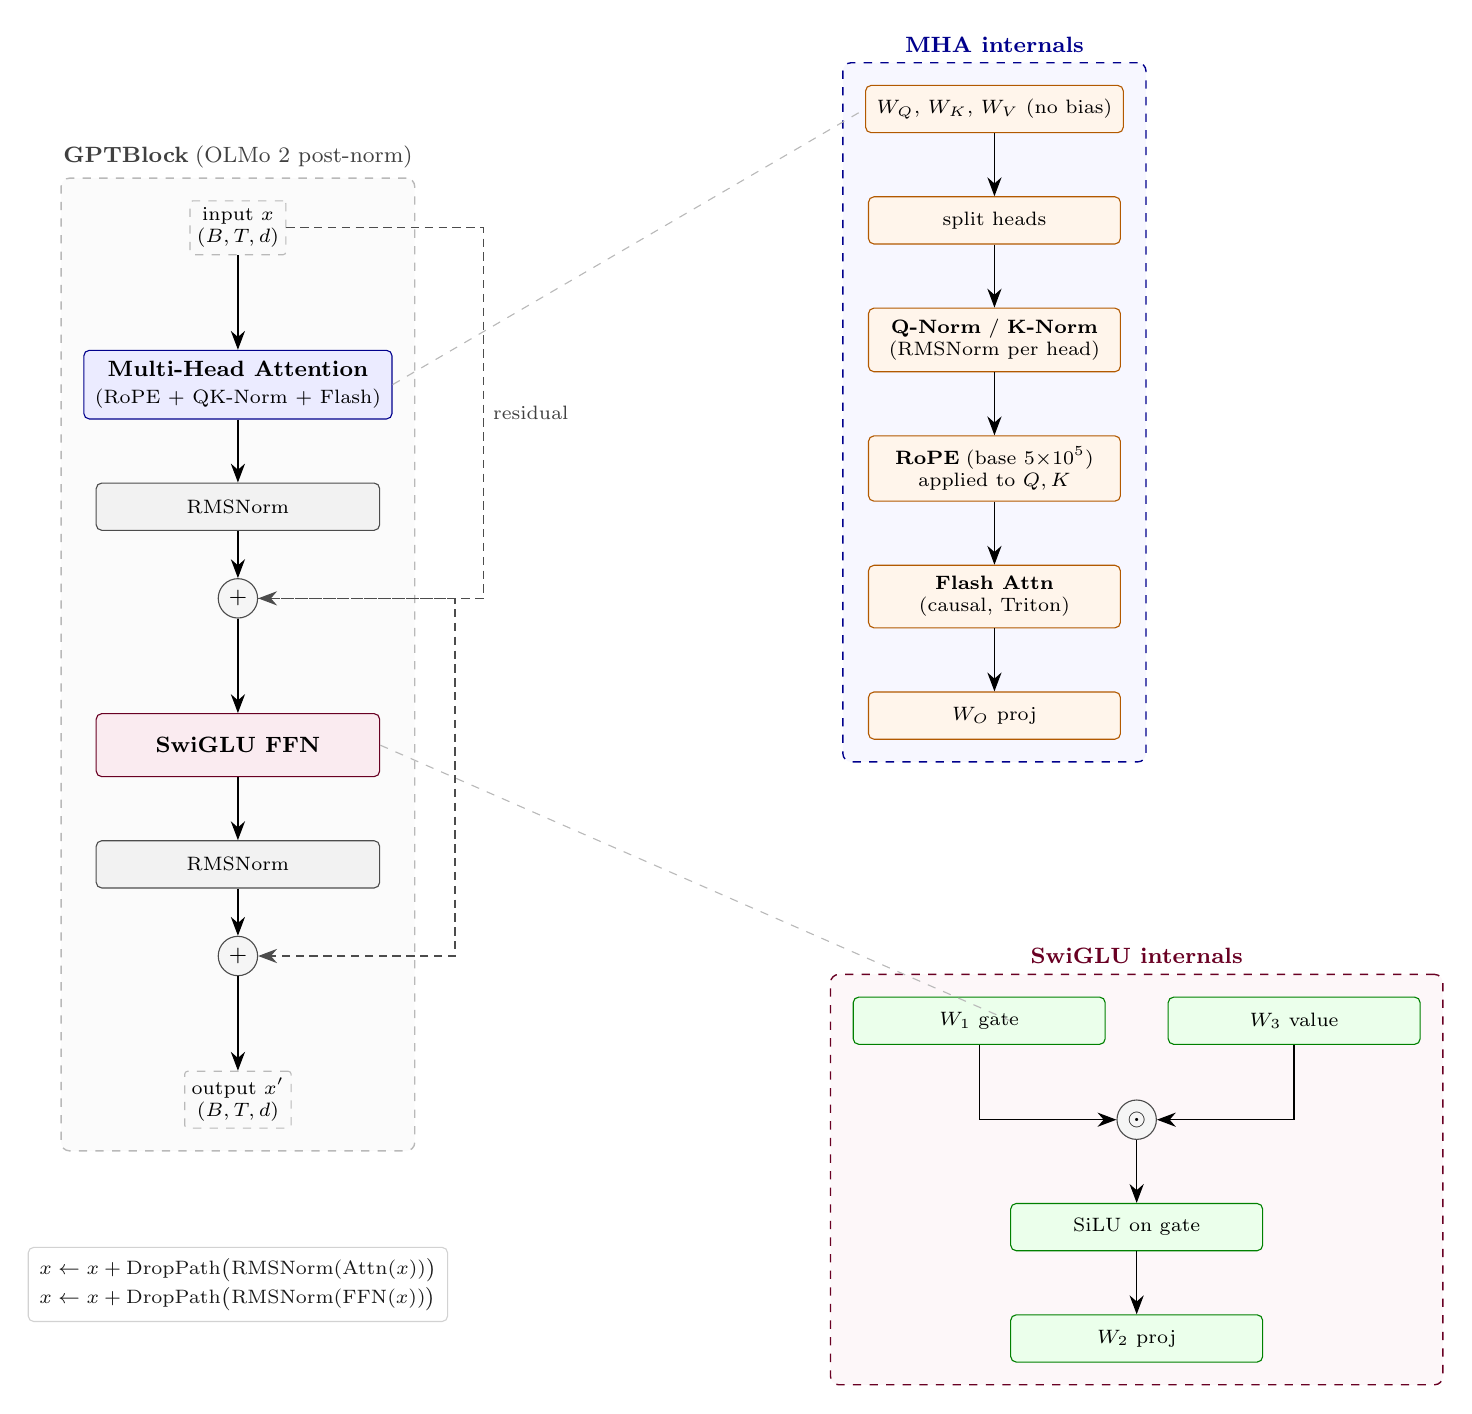
\begin{tikzpicture}[
    font=\footnotesize,
    >={Stealth[length=2.4mm]},
    node distance=8mm and 20mm, % 再次大幅增加全局间距
    blk/.style    ={draw, rounded corners=2pt, align=center,
                    minimum height=8mm, inner sep=4pt, line width=0.4pt},
    attn/.style   ={blk, fill=blue!8,    draw=blue!55!black, minimum width=36mm},
    ffn/.style    ={blk, fill=purple!8,  draw=purple!55!black, minimum width=36mm},
    norm/.style   ={blk, fill=gray!10,   draw=gray!60!black, minimum width=36mm,
                    minimum height=6mm, font=\scriptsize},
    sub/.style    ={blk, fill=orange!8,  draw=orange!70!black,
                    minimum width=32mm, minimum height=6mm, font=\scriptsize},
    subg/.style   ={blk, fill=green!8,   draw=green!50!black,
                    minimum width=32mm, minimum height=6mm, font=\scriptsize},
    io/.style     ={draw, dashed, rounded corners=1pt, align=center,
                    fill=gray!4, draw=gray!55, font=\scriptsize, inner sep=2.5pt},
    op/.style     ={draw, circle, inner sep=0.6pt, minimum size=5mm,
                    fill=gray!8, draw=gray!60!black, font=\footnotesize},
    pillar/.style ={draw, rounded corners=3pt, dashed, line width=0.5pt,
                    inner sep=8pt}, % 再次增加pillar内边距
    flow/.style   ={->, line width=0.5pt},
    res/.style    ={->, line width=0.5pt, gray!60!black, densely dashed},
]

% ============================================================
% MAIN COLUMN — GPTBlock 主流程
% ============================================================
\node[io] (xin) {input $x$\\$(B,T,d)$};

% --- Attention sublayer ---
\node[attn, below=12mm of xin] (attnblk)
    {\textbf{Multi-Head Attention}\\\scriptsize (RoPE + QK-Norm + Flash)};
\node[norm, below=of attnblk] (norm1) {RMSNorm};
\node[op, below=6mm of norm1] (add1) {$+$};

% --- FFN sublayer ---
\node[ffn, below=12mm of add1] (ffnblk)
    {\textbf{SwiGLU FFN}};
\node[norm, below=of ffnblk] (norm2) {RMSNorm};
\node[op, below=6mm of norm2] (add2) {$+$};

\node[io, below=12mm of add2] (xout) {output $x'$\\$(B,T,d)$};

% main flow
\draw[flow] (xin)     -- (attnblk);
\draw[flow] (attnblk) -- (norm1);
\draw[flow] (norm1)   -- (add1);
\draw[flow] (add1)    -- (ffnblk);
\draw[flow] (ffnblk)  -- (norm2);
\draw[flow] (norm2)   -- (add2);
\draw[flow] (add2)    -- (xout);

% residual connections (skip around each sublayer)
\draw[res] (xin.east) -| ++(25mm,0) |- (add1.east)
    node[pos=0.25, right, font=\scriptsize, gray!50!black] {residual};
\draw[res] (add1.east) -| ++(25mm,0) |- (add2.east);

% ============================================================
% RIGHT PANEL #1 — MHA internals (大幅上移，完全脱离SwiGLU区域)
% ============================================================
\node[sub, right=60mm of attnblk, yshift=35mm]   (qkv)   {$W_Q,\,W_K,\,W_V$ (no bias)};
\node[sub, below=of qkv]                         (split) {split heads};
\node[sub, below=of split]                       (qknorm){\textbf{Q-Norm} / \textbf{K-Norm}\\(RMSNorm per head)};
\node[sub, below=of qknorm]                      (rope)  {\textbf{RoPE}\;(base $5{\times}10^5$)\\applied to $Q,K$};
\node[sub, below=of rope]                        (flash) {\textbf{Flash Attn}\\(causal, Triton)};
\node[sub, below=of flash]                       (wo)    {$W_O$ proj};

\draw[flow] (qkv)    -- (split);
\draw[flow] (split)  -- (qknorm);
\draw[flow] (qknorm) -- (rope);
\draw[flow] (rope)   -- (flash);
\draw[flow] (flash)  -- (wo);

% 引线 attnblk → 展开
\draw[dashed, gray!55] (attnblk.east) -- (qkv.west);

% ============================================================
% RIGHT PANEL #2 — SwiGLU internals (大幅下移，与MHA完全分离)
% ============================================================
\node[subg, right=60mm of ffnblk, yshift=-35mm]    (w1)    {$W_1$ gate};
\node[subg, right=60mm of ffnblk, yshift=-35mm, xshift=40mm] (w3) {$W_3$ value};
\node[op,   below=10mm of $(w1)!0.5!(w3)$]         (had)   {$\odot$};
\node[subg, below=8mm of had]                     (silu)  {SiLU on gate};
\node[subg, below=8mm of silu]                        (w2)    {$W_2$ proj};

\draw[flow] (w1)   |- (had.west);
\draw[flow] (w3)   |- (had.east);
\draw[flow] (had)  -- (silu);
\draw[flow] (silu) -- (w2);

\draw[dashed, gray!55] (ffnblk.east) -- ($(w1.west)!0.5!(w3.west)$);

% ============================================================
% PILLARS (重新计算范围，确保无重叠)
% ============================================================
\begin{pgfonlayer}{background}
  \node[pillar, draw=blue!55!black, fill=blue!3,
        fit=(qkv)(split)(qknorm)(rope)(flash)(wo),
        label={[blue!55!black]above:\textbf{MHA internals}}]
        (mhabox) {};
  \node[pillar, draw=purple!55!black, fill=purple!3,
        fit=(w1)(w3)(had)(silu)(w2),
        label={[purple!55!black]above:\textbf{SwiGLU internals}}]
        (ffnbox) {};
  \node[pillar, draw=gray!55, fill=gray!3,
        fit=(xin)(attnblk)(norm1)(add1)(ffnblk)(norm2)(add2)(xout),
        label={[gray!50!black]above:\textbf{GPTBlock}\;(OLMo 2 post-norm)}]
        (mainbox) {};
\end{pgfonlayer}

% ============================================================
% FORMULA (左下角，位置微调)
% ============================================================
\node[draw, rounded corners=2pt, align=left, font=\scriptsize,
      fill=white, draw=gray!35, text opacity=0.9, inner sep=4pt,
      below=15mm of xout, anchor=north] (formula)
{$x \leftarrow x + \mathrm{DropPath}\bigl(\mathrm{RMSNorm}(\mathrm{Attn}(x))\bigr)$\\[1pt]
 $x \leftarrow x + \mathrm{DropPath}\bigl(\mathrm{RMSNorm}(\mathrm{FFN}(x))\bigr)$};

\end{tikzpicture}
\end{document}
%
% 对应 src/mdlic/models/layers.py:GPTBlock (line 366)
%   x = x + DropPath(RMSNorm(Attn(x)))    -- OLMo 2 post-norm，注意 Norm 在 sublayer 之后
%   x = x + DropPath(RMSNorm(FFN(x)))
\documentclass[tikz,border=8pt]{standalone}
\usepackage{tikz}
\usepackage{amsmath,amssymb}
\usetikzlibrary{positioning,arrows.meta,calc,fit,backgrounds,shapes.geometric}

\begin{document}
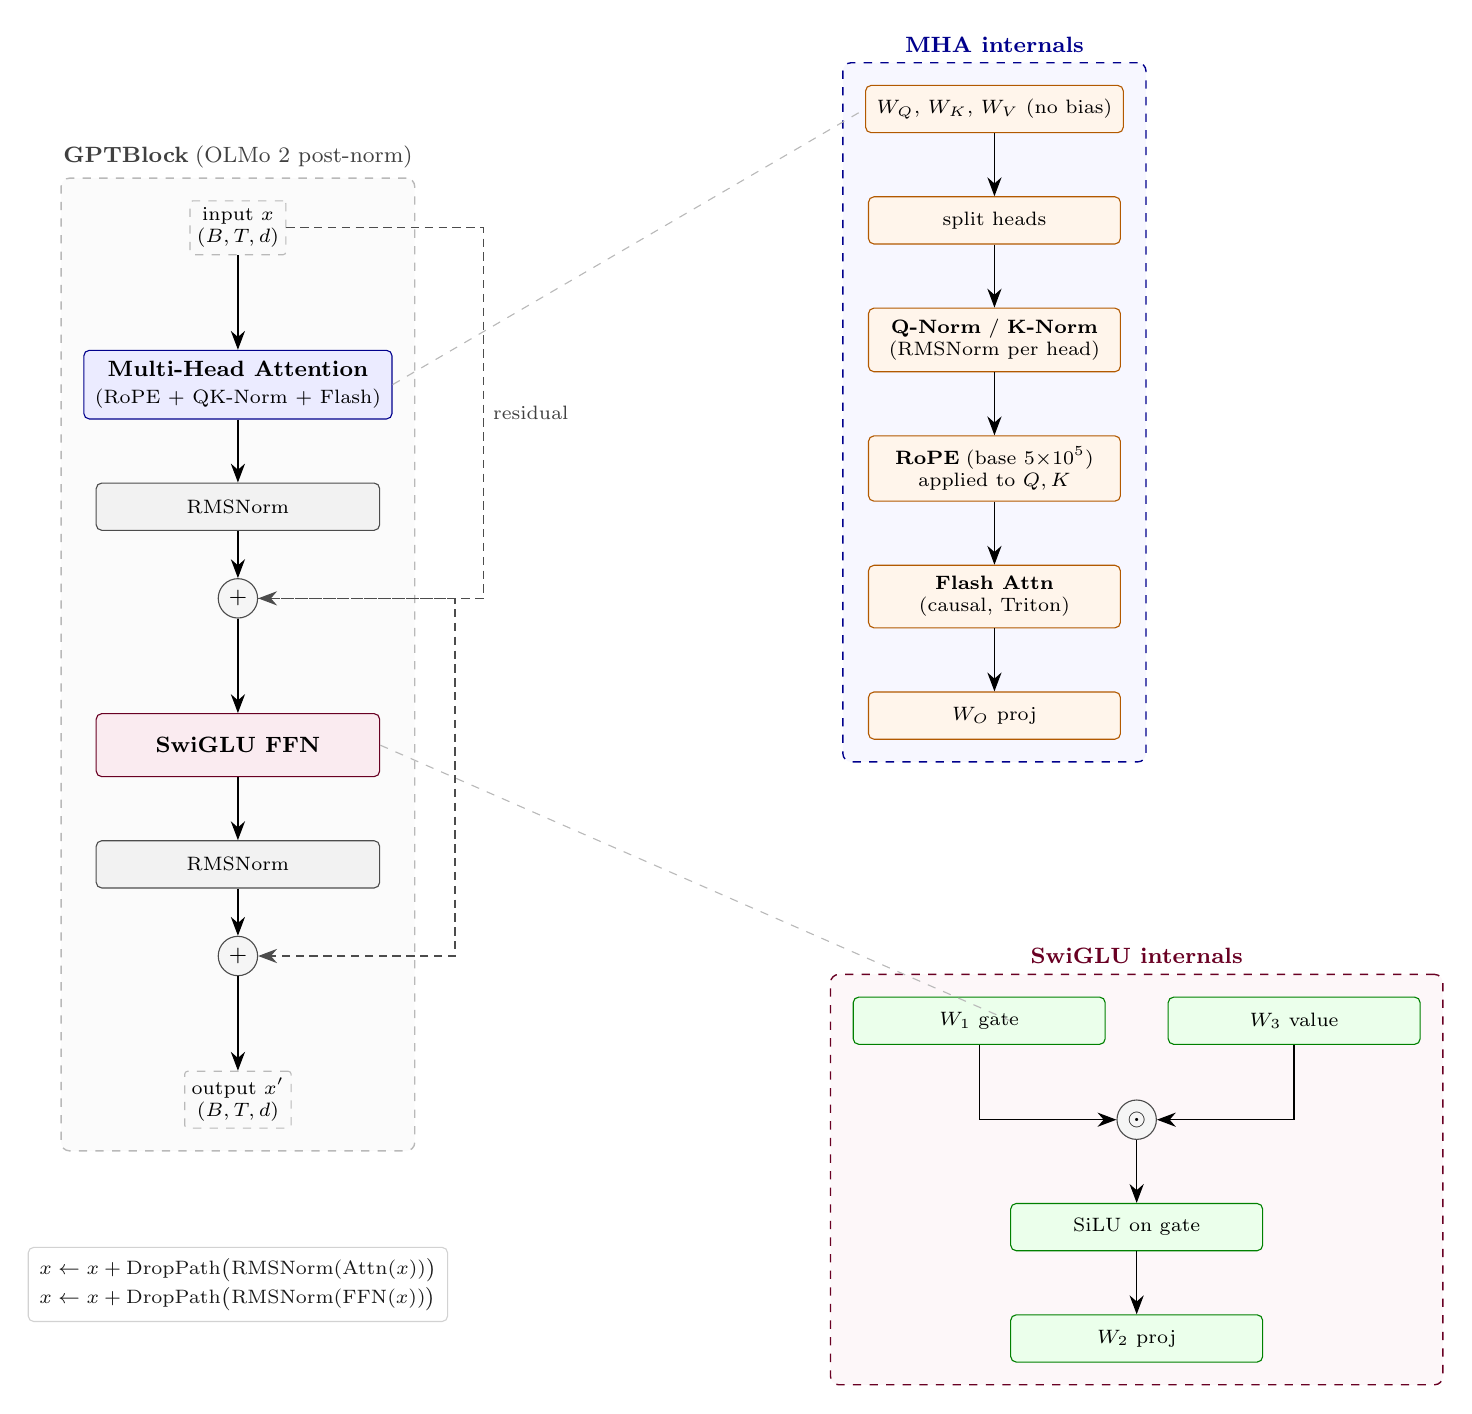
\begin{tikzpicture}[
    font=\footnotesize,
    >={Stealth[length=2.4mm]},
    node distance=8mm and 20mm, % 再次大幅增加全局间距
    blk/.style    ={draw, rounded corners=2pt, align=center,
                    minimum height=8mm, inner sep=4pt, line width=0.4pt},
    attn/.style   ={blk, fill=blue!8,    draw=blue!55!black, minimum width=36mm},
    ffn/.style    ={blk, fill=purple!8,  draw=purple!55!black, minimum width=36mm},
    norm/.style   ={blk, fill=gray!10,   draw=gray!60!black, minimum width=36mm,
                    minimum height=6mm, font=\scriptsize},
    sub/.style    ={blk, fill=orange!8,  draw=orange!70!black,
                    minimum width=32mm, minimum height=6mm, font=\scriptsize},
    subg/.style   ={blk, fill=green!8,   draw=green!50!black,
                    minimum width=32mm, minimum height=6mm, font=\scriptsize},
    io/.style     ={draw, dashed, rounded corners=1pt, align=center,
                    fill=gray!4, draw=gray!55, font=\scriptsize, inner sep=2.5pt},
    op/.style     ={draw, circle, inner sep=0.6pt, minimum size=5mm,
                    fill=gray!8, draw=gray!60!black, font=\footnotesize},
    pillar/.style ={draw, rounded corners=3pt, dashed, line width=0.5pt,
                    inner sep=8pt}, % 再次增加pillar内边距
    flow/.style   ={->, line width=0.5pt},
    res/.style    ={->, line width=0.5pt, gray!60!black, densely dashed},
]

% ============================================================
% MAIN COLUMN — GPTBlock 主流程
% ============================================================
\node[io] (xin) {input $x$\\$(B,T,d)$};

% --- Attention sublayer ---
\node[attn, below=12mm of xin] (attnblk)
    {\textbf{Multi-Head Attention}\\\scriptsize (RoPE + QK-Norm + Flash)};
\node[norm, below=of attnblk] (norm1) {RMSNorm};
\node[op, below=6mm of norm1] (add1) {$+$};

% --- FFN sublayer ---
\node[ffn, below=12mm of add1] (ffnblk)
    {\textbf{SwiGLU FFN}};
\node[norm, below=of ffnblk] (norm2) {RMSNorm};
\node[op, below=6mm of norm2] (add2) {$+$};

\node[io, below=12mm of add2] (xout) {output $x'$\\$(B,T,d)$};

% main flow
\draw[flow] (xin)     -- (attnblk);
\draw[flow] (attnblk) -- (norm1);
\draw[flow] (norm1)   -- (add1);
\draw[flow] (add1)    -- (ffnblk);
\draw[flow] (ffnblk)  -- (norm2);
\draw[flow] (norm2)   -- (add2);
\draw[flow] (add2)    -- (xout);

% residual connections (skip around each sublayer)
\draw[res] (xin.east) -| ++(25mm,0) |- (add1.east)
    node[pos=0.25, right, font=\scriptsize, gray!50!black] {residual};
\draw[res] (add1.east) -| ++(25mm,0) |- (add2.east);

% ============================================================
% RIGHT PANEL #1 — MHA internals (大幅上移，完全脱离SwiGLU区域)
% ============================================================
\node[sub, right=60mm of attnblk, yshift=35mm]   (qkv)   {$W_Q,\,W_K,\,W_V$ (no bias)};
\node[sub, below=of qkv]                         (split) {split heads};
\node[sub, below=of split]                       (qknorm){\textbf{Q-Norm} / \textbf{K-Norm}\\(RMSNorm per head)};
\node[sub, below=of qknorm]                      (rope)  {\textbf{RoPE}\;(base $5{\times}10^5$)\\applied to $Q,K$};
\node[sub, below=of rope]                        (flash) {\textbf{Flash Attn}\\(causal, Triton)};
\node[sub, below=of flash]                       (wo)    {$W_O$ proj};

\draw[flow] (qkv)    -- (split);
\draw[flow] (split)  -- (qknorm);
\draw[flow] (qknorm) -- (rope);
\draw[flow] (rope)   -- (flash);
\draw[flow] (flash)  -- (wo);

% 引线 attnblk → 展开
\draw[dashed, gray!55] (attnblk.east) -- (qkv.west);

% ============================================================
% RIGHT PANEL #2 — SwiGLU internals (大幅下移，与MHA完全分离)
% ============================================================
\node[subg, right=60mm of ffnblk, yshift=-35mm]    (w1)    {$W_1$ gate};
\node[subg, right=60mm of ffnblk, yshift=-35mm, xshift=40mm] (w3) {$W_3$ value};
\node[op,   below=10mm of $(w1)!0.5!(w3)$]         (had)   {$\odot$};
\node[subg, below=8mm of had]                     (silu)  {SiLU on gate};
\node[subg, below=8mm of silu]                        (w2)    {$W_2$ proj};

\draw[flow] (w1)   |- (had.west);
\draw[flow] (w3)   |- (had.east);
\draw[flow] (had)  -- (silu);
\draw[flow] (silu) -- (w2);

\draw[dashed, gray!55] (ffnblk.east) -- ($(w1.west)!0.5!(w3.west)$);

% ============================================================
% PILLARS (重新计算范围，确保无重叠)
% ============================================================
\begin{pgfonlayer}{background}
  \node[pillar, draw=blue!55!black, fill=blue!3,
        fit=(qkv)(split)(qknorm)(rope)(flash)(wo),
        label={[blue!55!black]above:\textbf{MHA internals}}]
        (mhabox) {};
  \node[pillar, draw=purple!55!black, fill=purple!3,
        fit=(w1)(w3)(had)(silu)(w2),
        label={[purple!55!black]above:\textbf{SwiGLU internals}}]
        (ffnbox) {};
  \node[pillar, draw=gray!55, fill=gray!3,
        fit=(xin)(attnblk)(norm1)(add1)(ffnblk)(norm2)(add2)(xout),
        label={[gray!50!black]above:\textbf{GPTBlock}\;(OLMo 2 post-norm)}]
        (mainbox) {};
\end{pgfonlayer}

% ============================================================
% FORMULA (左下角，位置微调)
% ============================================================
\node[draw, rounded corners=2pt, align=left, font=\scriptsize,
      fill=white, draw=gray!35, text opacity=0.9, inner sep=4pt,
      below=15mm of xout, anchor=north] (formula)
{$x \leftarrow x + \mathrm{DropPath}\bigl(\mathrm{RMSNorm}(\mathrm{Attn}(x))\bigr)$\\[1pt]
 $x \leftarrow x + \mathrm{DropPath}\bigl(\mathrm{RMSNorm}(\mathrm{FFN}(x))\bigr)$};

\end{tikzpicture}
\end{document}
%
% 对应 src/mdlic/models/layers.py:GPTBlock (line 366)
%   x = x + DropPath(RMSNorm(Attn(x)))    -- OLMo 2 post-norm，注意 Norm 在 sublayer 之后
%   x = x + DropPath(RMSNorm(FFN(x)))
\documentclass[tikz,border=8pt]{standalone}
\usepackage{tikz}
\usepackage{amsmath,amssymb}
\usetikzlibrary{positioning,arrows.meta,calc,fit,backgrounds,shapes.geometric}

\begin{document}
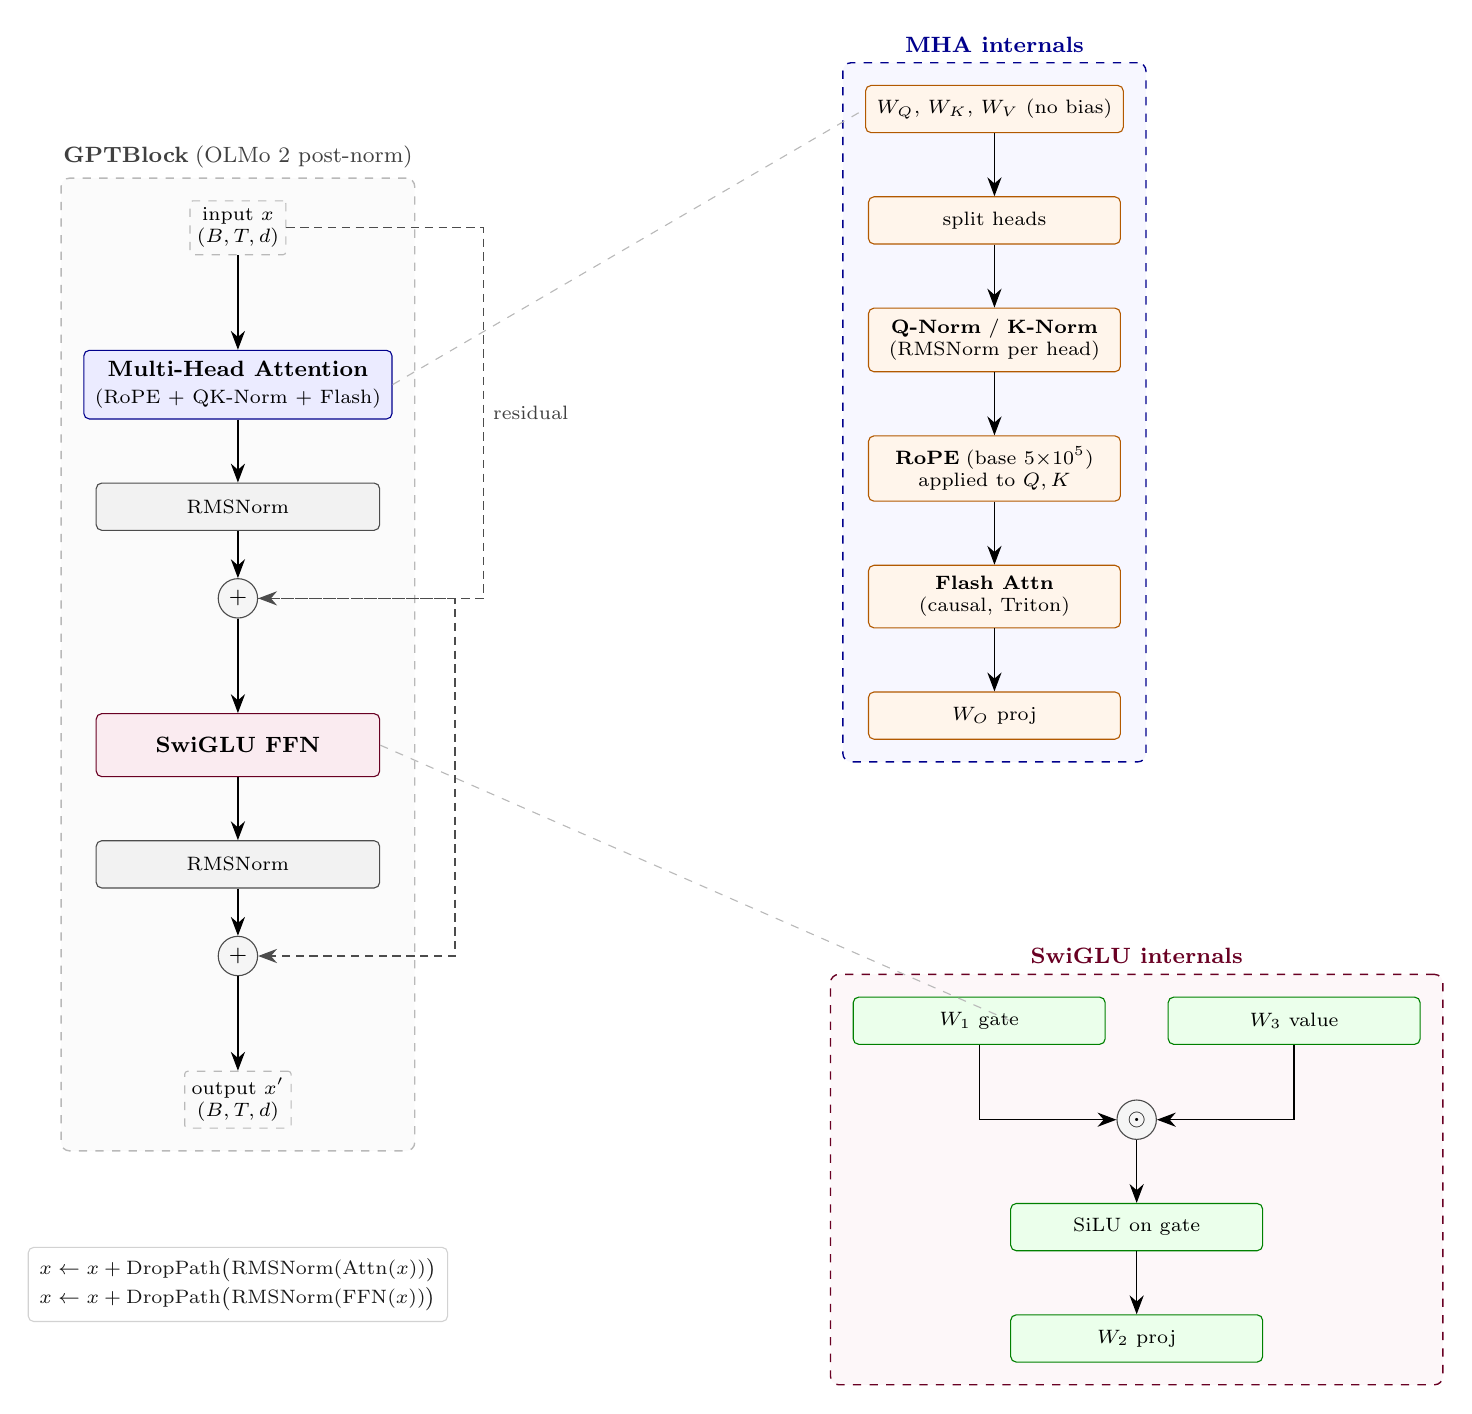
\begin{tikzpicture}[
    font=\footnotesize,
    >={Stealth[length=2.4mm]},
    node distance=8mm and 20mm, % 再次大幅增加全局间距
    blk/.style    ={draw, rounded corners=2pt, align=center,
                    minimum height=8mm, inner sep=4pt, line width=0.4pt},
    attn/.style   ={blk, fill=blue!8,    draw=blue!55!black, minimum width=36mm},
    ffn/.style    ={blk, fill=purple!8,  draw=purple!55!black, minimum width=36mm},
    norm/.style   ={blk, fill=gray!10,   draw=gray!60!black, minimum width=36mm,
                    minimum height=6mm, font=\scriptsize},
    sub/.style    ={blk, fill=orange!8,  draw=orange!70!black,
                    minimum width=32mm, minimum height=6mm, font=\scriptsize},
    subg/.style   ={blk, fill=green!8,   draw=green!50!black,
                    minimum width=32mm, minimum height=6mm, font=\scriptsize},
    io/.style     ={draw, dashed, rounded corners=1pt, align=center,
                    fill=gray!4, draw=gray!55, font=\scriptsize, inner sep=2.5pt},
    op/.style     ={draw, circle, inner sep=0.6pt, minimum size=5mm,
                    fill=gray!8, draw=gray!60!black, font=\footnotesize},
    pillar/.style ={draw, rounded corners=3pt, dashed, line width=0.5pt,
                    inner sep=8pt}, % 再次增加pillar内边距
    flow/.style   ={->, line width=0.5pt},
    res/.style    ={->, line width=0.5pt, gray!60!black, densely dashed},
]

% ============================================================
% MAIN COLUMN — GPTBlock 主流程
% ============================================================
\node[io] (xin) {input $x$\\$(B,T,d)$};

% --- Attention sublayer ---
\node[attn, below=12mm of xin] (attnblk)
    {\textbf{Multi-Head Attention}\\\scriptsize (RoPE + QK-Norm + Flash)};
\node[norm, below=of attnblk] (norm1) {RMSNorm};
\node[op, below=6mm of norm1] (add1) {$+$};

% --- FFN sublayer ---
\node[ffn, below=12mm of add1] (ffnblk)
    {\textbf{SwiGLU FFN}};
\node[norm, below=of ffnblk] (norm2) {RMSNorm};
\node[op, below=6mm of norm2] (add2) {$+$};

\node[io, below=12mm of add2] (xout) {output $x'$\\$(B,T,d)$};

% main flow
\draw[flow] (xin)     -- (attnblk);
\draw[flow] (attnblk) -- (norm1);
\draw[flow] (norm1)   -- (add1);
\draw[flow] (add1)    -- (ffnblk);
\draw[flow] (ffnblk)  -- (norm2);
\draw[flow] (norm2)   -- (add2);
\draw[flow] (add2)    -- (xout);

% residual connections (skip around each sublayer)
\draw[res] (xin.east) -| ++(25mm,0) |- (add1.east)
    node[pos=0.25, right, font=\scriptsize, gray!50!black] {residual};
\draw[res] (add1.east) -| ++(25mm,0) |- (add2.east);

% ============================================================
% RIGHT PANEL #1 — MHA internals (大幅上移，完全脱离SwiGLU区域)
% ============================================================
\node[sub, right=60mm of attnblk, yshift=35mm]   (qkv)   {$W_Q,\,W_K,\,W_V$ (no bias)};
\node[sub, below=of qkv]                         (split) {split heads};
\node[sub, below=of split]                       (qknorm){\textbf{Q-Norm} / \textbf{K-Norm}\\(RMSNorm per head)};
\node[sub, below=of qknorm]                      (rope)  {\textbf{RoPE}\;(base $5{\times}10^5$)\\applied to $Q,K$};
\node[sub, below=of rope]                        (flash) {\textbf{Flash Attn}\\(causal, Triton)};
\node[sub, below=of flash]                       (wo)    {$W_O$ proj};

\draw[flow] (qkv)    -- (split);
\draw[flow] (split)  -- (qknorm);
\draw[flow] (qknorm) -- (rope);
\draw[flow] (rope)   -- (flash);
\draw[flow] (flash)  -- (wo);

% 引线 attnblk → 展开
\draw[dashed, gray!55] (attnblk.east) -- (qkv.west);

% ============================================================
% RIGHT PANEL #2 — SwiGLU internals (大幅下移，与MHA完全分离)
% ============================================================
\node[subg, right=60mm of ffnblk, yshift=-35mm]    (w1)    {$W_1$ gate};
\node[subg, right=60mm of ffnblk, yshift=-35mm, xshift=40mm] (w3) {$W_3$ value};
\node[op,   below=10mm of $(w1)!0.5!(w3)$]         (had)   {$\odot$};
\node[subg, below=8mm of had]                     (silu)  {SiLU on gate};
\node[subg, below=8mm of silu]                        (w2)    {$W_2$ proj};

\draw[flow] (w1)   |- (had.west);
\draw[flow] (w3)   |- (had.east);
\draw[flow] (had)  -- (silu);
\draw[flow] (silu) -- (w2);

\draw[dashed, gray!55] (ffnblk.east) -- ($(w1.west)!0.5!(w3.west)$);

% ============================================================
% PILLARS (重新计算范围，确保无重叠)
% ============================================================
\begin{pgfonlayer}{background}
  \node[pillar, draw=blue!55!black, fill=blue!3,
        fit=(qkv)(split)(qknorm)(rope)(flash)(wo),
        label={[blue!55!black]above:\textbf{MHA internals}}]
        (mhabox) {};
  \node[pillar, draw=purple!55!black, fill=purple!3,
        fit=(w1)(w3)(had)(silu)(w2),
        label={[purple!55!black]above:\textbf{SwiGLU internals}}]
        (ffnbox) {};
  \node[pillar, draw=gray!55, fill=gray!3,
        fit=(xin)(attnblk)(norm1)(add1)(ffnblk)(norm2)(add2)(xout),
        label={[gray!50!black]above:\textbf{GPTBlock}\;(OLMo 2 post-norm)}]
        (mainbox) {};
\end{pgfonlayer}

% ============================================================
% FORMULA (左下角，位置微调)
% ============================================================
\node[draw, rounded corners=2pt, align=left, font=\scriptsize,
      fill=white, draw=gray!35, text opacity=0.9, inner sep=4pt,
      below=15mm of xout, anchor=north] (formula)
{$x \leftarrow x + \mathrm{DropPath}\bigl(\mathrm{RMSNorm}(\mathrm{Attn}(x))\bigr)$\\[1pt]
 $x \leftarrow x + \mathrm{DropPath}\bigl(\mathrm{RMSNorm}(\mathrm{FFN}(x))\bigr)$};

\end{tikzpicture}
\end{document}
%
% 对应 src/mdlic/models/layers.py:GPTBlock (line 366)
%   x = x + DropPath(RMSNorm(Attn(x)))    -- OLMo 2 post-norm，注意 Norm 在 sublayer 之后
%   x = x + DropPath(RMSNorm(FFN(x)))
\documentclass[tikz,border=8pt]{standalone}
\usepackage{tikz}
\usepackage{amsmath,amssymb}
\usetikzlibrary{positioning,arrows.meta,calc,fit,backgrounds,shapes.geometric}

\begin{document}
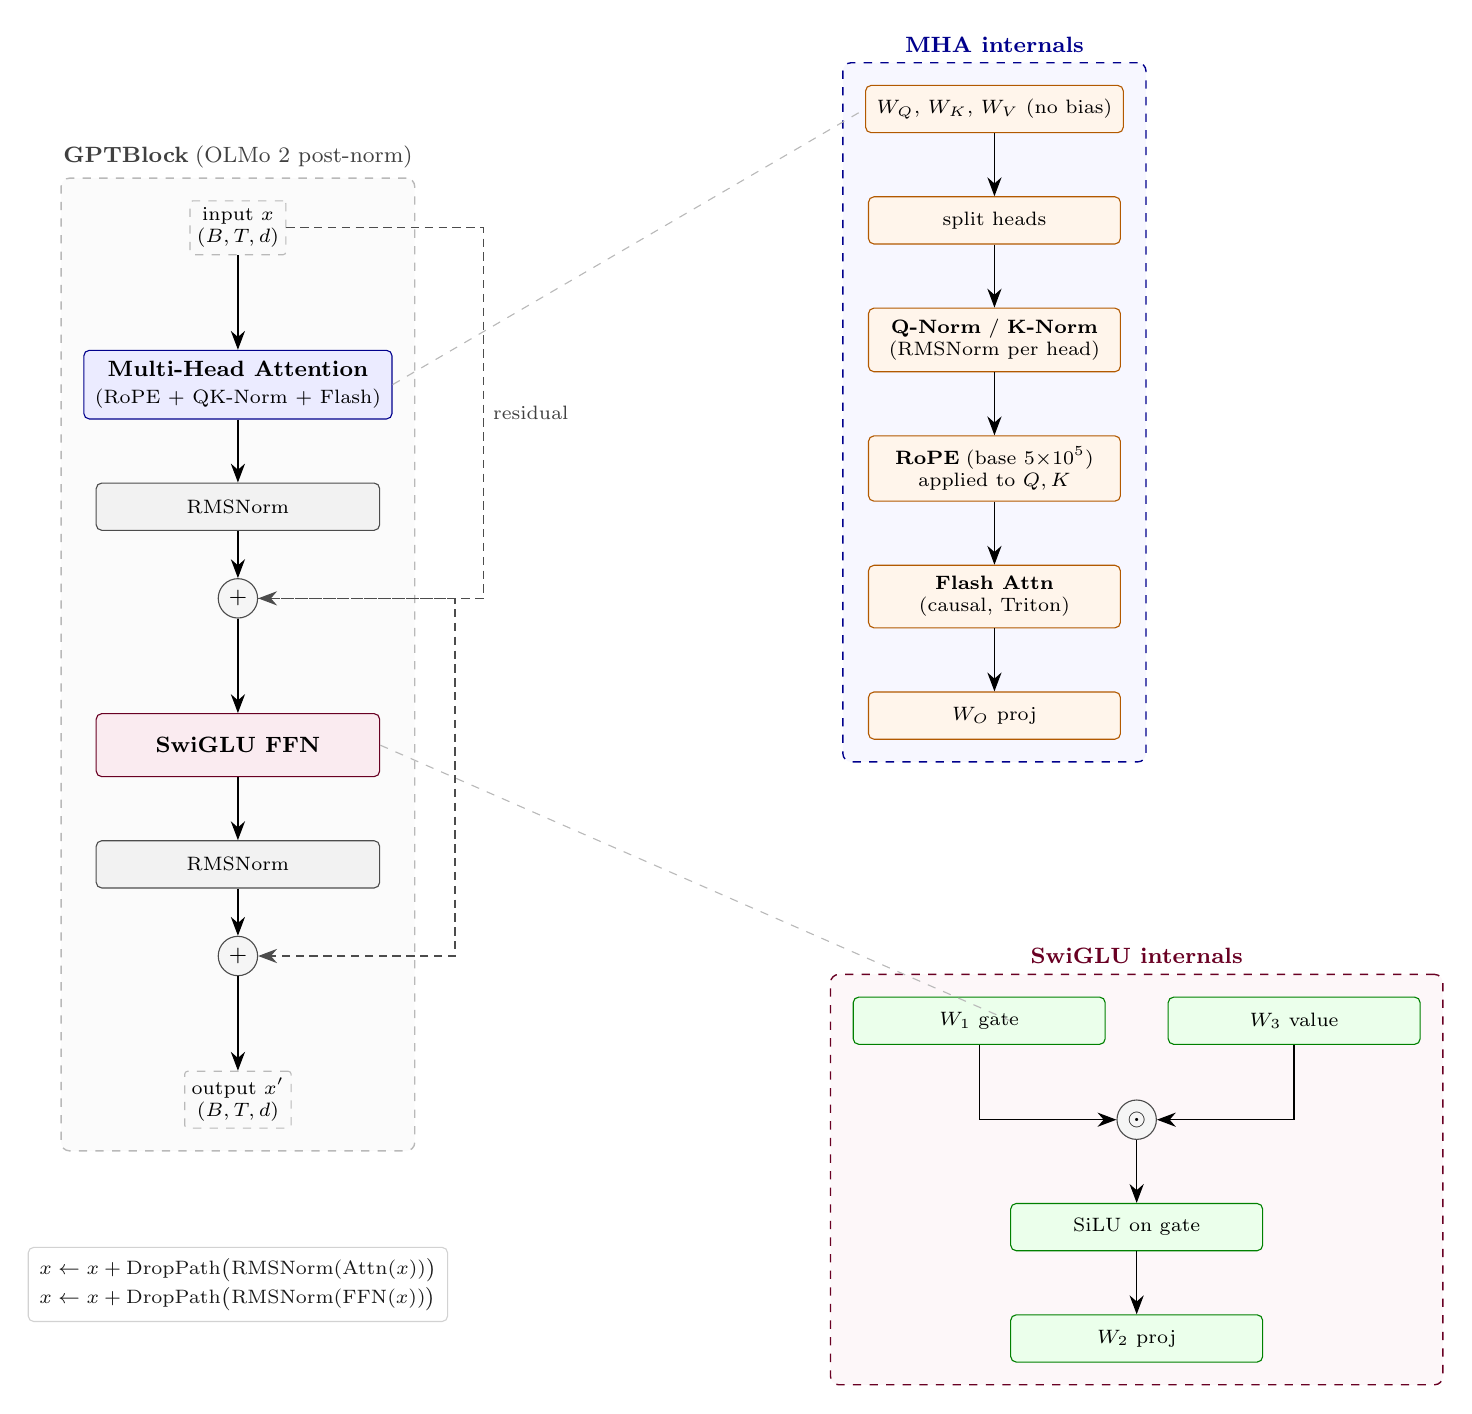
\begin{tikzpicture}[
    font=\footnotesize,
    >={Stealth[length=2.4mm]},
    node distance=8mm and 20mm, % 再次大幅增加全局间距
    blk/.style    ={draw, rounded corners=2pt, align=center,
                    minimum height=8mm, inner sep=4pt, line width=0.4pt},
    attn/.style   ={blk, fill=blue!8,    draw=blue!55!black, minimum width=36mm},
    ffn/.style    ={blk, fill=purple!8,  draw=purple!55!black, minimum width=36mm},
    norm/.style   ={blk, fill=gray!10,   draw=gray!60!black, minimum width=36mm,
                    minimum height=6mm, font=\scriptsize},
    sub/.style    ={blk, fill=orange!8,  draw=orange!70!black,
                    minimum width=32mm, minimum height=6mm, font=\scriptsize},
    subg/.style   ={blk, fill=green!8,   draw=green!50!black,
                    minimum width=32mm, minimum height=6mm, font=\scriptsize},
    io/.style     ={draw, dashed, rounded corners=1pt, align=center,
                    fill=gray!4, draw=gray!55, font=\scriptsize, inner sep=2.5pt},
    op/.style     ={draw, circle, inner sep=0.6pt, minimum size=5mm,
                    fill=gray!8, draw=gray!60!black, font=\footnotesize},
    pillar/.style ={draw, rounded corners=3pt, dashed, line width=0.5pt,
                    inner sep=8pt}, % 再次增加pillar内边距
    flow/.style   ={->, line width=0.5pt},
    res/.style    ={->, line width=0.5pt, gray!60!black, densely dashed},
]

% ============================================================
% MAIN COLUMN — GPTBlock 主流程
% ============================================================
\node[io] (xin) {input $x$\\$(B,T,d)$};

% --- Attention sublayer ---
\node[attn, below=12mm of xin] (attnblk)
    {\textbf{Multi-Head Attention}\\\scriptsize (RoPE + QK-Norm + Flash)};
\node[norm, below=of attnblk] (norm1) {RMSNorm};
\node[op, below=6mm of norm1] (add1) {$+$};

% --- FFN sublayer ---
\node[ffn, below=12mm of add1] (ffnblk)
    {\textbf{SwiGLU FFN}};
\node[norm, below=of ffnblk] (norm2) {RMSNorm};
\node[op, below=6mm of norm2] (add2) {$+$};

\node[io, below=12mm of add2] (xout) {output $x'$\\$(B,T,d)$};

% main flow
\draw[flow] (xin)     -- (attnblk);
\draw[flow] (attnblk) -- (norm1);
\draw[flow] (norm1)   -- (add1);
\draw[flow] (add1)    -- (ffnblk);
\draw[flow] (ffnblk)  -- (norm2);
\draw[flow] (norm2)   -- (add2);
\draw[flow] (add2)    -- (xout);

% residual connections (skip around each sublayer)
\draw[res] (xin.east) -| ++(25mm,0) |- (add1.east)
    node[pos=0.25, right, font=\scriptsize, gray!50!black] {residual};
\draw[res] (add1.east) -| ++(25mm,0) |- (add2.east);

% ============================================================
% RIGHT PANEL #1 — MHA internals (大幅上移，完全脱离SwiGLU区域)
% ============================================================
\node[sub, right=60mm of attnblk, yshift=35mm]   (qkv)   {$W_Q,\,W_K,\,W_V$ (no bias)};
\node[sub, below=of qkv]                         (split) {split heads};
\node[sub, below=of split]                       (qknorm){\textbf{Q-Norm} / \textbf{K-Norm}\\(RMSNorm per head)};
\node[sub, below=of qknorm]                      (rope)  {\textbf{RoPE}\;(base $5{\times}10^5$)\\applied to $Q,K$};
\node[sub, below=of rope]                        (flash) {\textbf{Flash Attn}\\(causal, Triton)};
\node[sub, below=of flash]                       (wo)    {$W_O$ proj};

\draw[flow] (qkv)    -- (split);
\draw[flow] (split)  -- (qknorm);
\draw[flow] (qknorm) -- (rope);
\draw[flow] (rope)   -- (flash);
\draw[flow] (flash)  -- (wo);

% 引线 attnblk → 展开
\draw[dashed, gray!55] (attnblk.east) -- (qkv.west);

% ============================================================
% RIGHT PANEL #2 — SwiGLU internals (大幅下移，与MHA完全分离)
% ============================================================
\node[subg, right=60mm of ffnblk, yshift=-35mm]    (w1)    {$W_1$ gate};
\node[subg, right=60mm of ffnblk, yshift=-35mm, xshift=40mm] (w3) {$W_3$ value};
\node[op,   below=10mm of $(w1)!0.5!(w3)$]         (had)   {$\odot$};
\node[subg, below=8mm of had]                     (silu)  {SiLU on gate};
\node[subg, below=8mm of silu]                        (w2)    {$W_2$ proj};

\draw[flow] (w1)   |- (had.west);
\draw[flow] (w3)   |- (had.east);
\draw[flow] (had)  -- (silu);
\draw[flow] (silu) -- (w2);

\draw[dashed, gray!55] (ffnblk.east) -- ($(w1.west)!0.5!(w3.west)$);

% ============================================================
% PILLARS (重新计算范围，确保无重叠)
% ============================================================
\begin{pgfonlayer}{background}
  \node[pillar, draw=blue!55!black, fill=blue!3,
        fit=(qkv)(split)(qknorm)(rope)(flash)(wo),
        label={[blue!55!black]above:\textbf{MHA internals}}]
        (mhabox) {};
  \node[pillar, draw=purple!55!black, fill=purple!3,
        fit=(w1)(w3)(had)(silu)(w2),
        label={[purple!55!black]above:\textbf{SwiGLU internals}}]
        (ffnbox) {};
  \node[pillar, draw=gray!55, fill=gray!3,
        fit=(xin)(attnblk)(norm1)(add1)(ffnblk)(norm2)(add2)(xout),
        label={[gray!50!black]above:\textbf{GPTBlock}\;(OLMo 2 post-norm)}]
        (mainbox) {};
\end{pgfonlayer}

% ============================================================
% FORMULA (左下角，位置微调)
% ============================================================
\node[draw, rounded corners=2pt, align=left, font=\scriptsize,
      fill=white, draw=gray!35, text opacity=0.9, inner sep=4pt,
      below=15mm of xout, anchor=north] (formula)
{$x \leftarrow x + \mathrm{DropPath}\bigl(\mathrm{RMSNorm}(\mathrm{Attn}(x))\bigr)$\\[1pt]
 $x \leftarrow x + \mathrm{DropPath}\bigl(\mathrm{RMSNorm}(\mathrm{FFN}(x))\bigr)$};

\end{tikzpicture}
\end{document}